\chapter{\bh} \label{ch:blowhole}
  \begin{figure}[h]
    \centering
    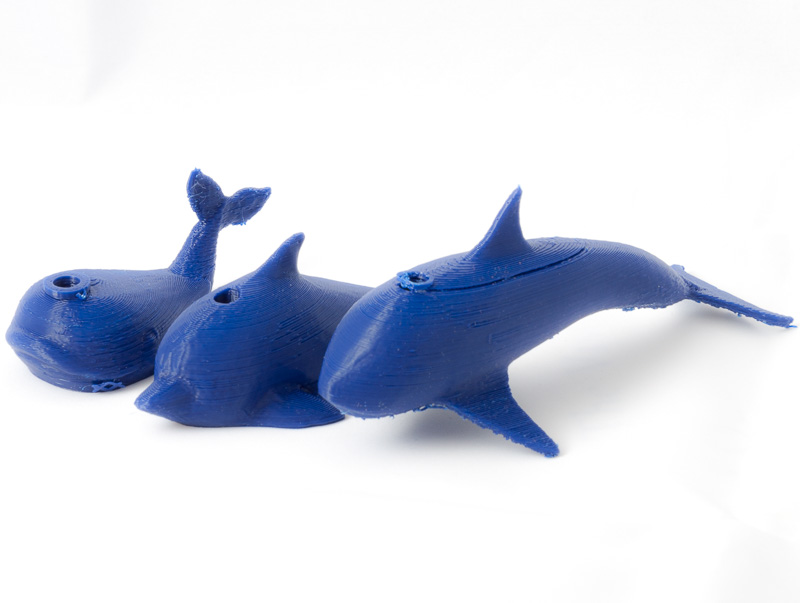
\includegraphics[width=0.33\textwidth]{print-and-play/blowhole/whales.jpg}
  \end{figure}

  \red{This page should explain how this paper ties together with the thesis}

  Lorem ipsum dolor sit amet, consectetur adipiscing elit. Proin ornare tempus
  risus id consectetur. In posuere ligula vel neque vehicula, nec rhoncus elit
  dapibus. Proin facilisis porttitor diam, vitae eleifend odio pellentesque id.
  Fusce eu semper erat, et malesuada massa. Duis laoreet sed neque a dictum.
  Quisque convallis accumsan justo sit amet vulputate. Integer auctor eros ac
  accumsan accumsan. Integer hendrerit urna id convallis tempus. Donec sem est,
  pretium sit amet gravida sed, suscipit a sapien. In eros nulla, bibendum nec
  malesuada in, sollicitudin a turpis. In egestas molestie iaculis. Cras eros
  quam, placerat eget eleifend sed, condimentum sit amet metus.

  Vivamus vitae lacinia lorem. Ut efficitur sollicitudin felis, et iaculis odio.
  Vestibulum sit amet nulla faucibus, egestas lorem quis, consequat neque.
  Integer vel laoreet ligula, a varius risus. Curabitur ac eleifend neque.
  Praesent sagittis volutpat libero, ut maximus arcu iaculis eu. Interdum et
  malesuada fames ac ante ipsum primis in faucibus. Sed maximus eros eget nisl
  scelerisque egestas. Mauris bibendum laoreet felis, cursus vestibulum enim
  condimentum nec.

  Nunc eget faucibus tortor. Fusce nisl lectus, congue in blandit non, pretium
  non metus. Fusce efficitur varius interdum. Phasellus ullamcorper gravida
  odio. Nulla accumsan purus risus, vitae porta nibh auctor non. Nulla varius
  eros scelerisque convallis maximus. In sed blandit augue. Proin commodo lacus
  ac orci suscipit porta. Aenean vitae libero pretium, convallis dui ut,
  accumsan leo. Morbi gravida scelerisque sapien quis fringilla. Aliquam nisl
  dolor, molestie eu nulla quis, malesuada pharetra velit. Vivamus porta dictum
  metus, vel molestie ex fermentum in. Vestibulum pellentesque vel ante vel
  feugiat. Integer mattis vitae libero nec laoreet. Aliquam erat volutpat. In
  hac habitasse platea dictumst.

  \newpage

  This chapter is based on the collaborative effort described below.

  \vfill

  \noindent
  \textbf{Title}\\
  \textit{Blowhole: Blowing-Activated Tags for Interactive 3D-Printed Models}

  \bigskip

  \noindent
  \textbf{Authors}\\
  \textit{\underline{Carlos E. Tejada}, Osamu Fujimoto, Zhiyuan Li, Daniel Ashbrook}

  \bigskip

  \noindent
  \textbf{DOI}\\
  \href{https://doi.org/10.20380/GI2018.18}{https://doi.org/10.20380/GI2018.18}


  \bigskip

  \noindent
  \textbf{Venue}\\
  \textit{Proceedings of the 44th Graphics Interface Conference}


  \bigskip

	\noindent
	\textbf{What was the role of the PhD student in designing the study?}\\
  \textit{The PhD student was the first author of the paper, and responsible
    of the described studies.}

	\bigskip

	\noindent
	\textbf{How did the PhD student participate in data collection and/or development of theory?}\\
  \textit{The PhD student was responisble for study implementation, execution,
    data collection, and theory development.}

	\bigskip

	\noindent
	\textbf{Which part of the manuscript did the PhD student write or contribute to?}\\
  \textit{The PhD student contributed to all parts of the manuscript.}

	\bigskip

	\noindent
	\textbf{Did the PhD student read and comment on the final manuscript?}\\
	\textit{Yes.}

  \bigskip
  \vfill

  \newpage

  \section{Abstract}
    Interactive 3D models have the potential to enhance accessibility and
    education, but can be complex and time-consuming to produce. We present
    \textit{\bh}, a technique for embedding blowing-activated tags into
    3D-printed models to add interactivity. Requiring no special printing
    techniques, components, or assembly and working on consumer-level 3D
    printers, \bh adds acoustically resonant cavities to the interior of a model
    with unobtrusive openings at the surface of the object. A gentle blow into a
    hole produces a unique sound that identifies the hole, allowing a computer
    to provide associated content. We describe the theory behind \bh,
    characterize the performance of different cavity parameters, and describe
    our implementation, including easy-to-use software to automatically embed
    blowholes into preexisting models. We illustrate \bh's potential with
    multiple working examples. 
  
  \section{Introduction}
    Adding interactivity to 3D-printed objects in an end-user-friendly way is a
    difficult undertaking. While doing so can enable a wealth of educational and
    accessibility applications (e.g., Figure \ref{fig:teaser}), adding
    interactivity can require extra components \cite{Savage:2013, Nappey:2014},
    special printing techniques \cite{Schmitz:2015, Bacher:2016, Peng:2015}, or
    large features that can disrupt the object's surface \cite{Harrison:2012kw,
    Ou:2016a, Savage:2015, Shi:2016} or make it larger \cite{Li:2016}. While
    such solutions can offer rich interaction possibilities such as buttons,
    touch sensitivity, and grasp sensing, many useful applications can be
    enabled by simply ``tagging'' 3D models, allowing a system to know what part
    of a model a user is interested in and respond with information.
    
    In this paper, we present \textit{\bh}, a system for unobtrusively tagging
    3D models or parts of models. Inspired by previous work in acoustic sensing,
    our system creates embedded, resonant cavities that a user gently blows into
    (Figure \ref{fig:teaser}). Different-sized cavities create sounds at
    different pitches that can be recognized by a computer. The main focus of
    \bh is to enable 3D-printing novices to create interactive objects which can
    be printed and immediately used with no during-print intervention,
    post-processing, or training necessary. The contributions of our work are as
    follows:

    \begin{itemize}
        \item a technique for embedding resonant cavities---printable on
          commodity 3D printers---into existing 3D models, which produce distinct
          pitches when blown into;
        \item characterization of the range of frequencies that can be generated
          and recognized by our system;
        \item a design environment which enables non-expert users to indicate
          areas which they wish annotated, and automatically generates and embeds
          appropriate cavities;
        \item and a user-independent system which recognizes the sounds of the
          user blowing into the cavities and plays back the associated
          annotations.
    \end{itemize}

  \section{Blowhole}
    \bh is based on the property of acoustic resonance; a familiar example is
    the sound created when blowing across the mouth of a bottle. \bh embeds
    cavities into 3D models, with tubular openings to the surface. Varying the
    volumes of the cavities and lengths of the tubes produces varying
    frequencies in response to gentle blowing into the holes, with the object
    held 5--10\,cm away from the mouth. Our system recognizes the characteristic
    sound of each hole, linking the blow sound to an action associated with the
    hole's location on the model. Our design tool allows a user to select the
    placement of holes on arbitrary 3D models and associate actions with each
    hole; the software then optimizes blowhole size and placement, providing a
    printer-ready file.
    
    The cavities used in \bh must satisfy several criteria: they must support
    sufficient variation in parameters to produce a range of frequencies when
    blown into; they must be sufficiently small to embed into models small
    enough to hold and manipulate; they should present a consistent hole
    appearance to the user; and they should be printable at any orientation and
    without support material on a consumer-grade printer.
    
    This last criterion poses the strongest limitation due to the limited
    ability of FDM\footnote{Fused Deposition Modeling---the most-common consumer
    printer technology} 3D printers to print with \textit{overhangs}---angles
    greater than 45° from gravity---and \textit{bridging}---printing
    material with nothing underneath it as a support. We experimented with a
    number of shapes. Simple tubes (as used, for example, in Whoosh
    \cite{Reyes:2016}) printed well at any orientation but quickly became too
    large to embed in smaller objects while supporting a range of frequencies.
    We tested several variations on shorter tubes connecting to larger cavities,
    which preserve a standard opening size but allow the production of a greater
    range of frequencies. We experimented with cavities shaped like spheres,
    cylinders, cylinders with cones on tops, cubes, and cubes with pyramids. The
    shape resulting in the best combination of clear sound and multi-orientation
    printability was a sphere with a tube connecting to the surface of the
    model. In the next section, we detail the theory behind the resonant
    properties of this structure.

    \subsection{Cavity Resonator Theory}
      \bh operates on the principle of acoustic resonance, where particular
      frequencies are amplified or attenuated due to the physical properties of
      a cavity. \bh uses spherical cavities inside a 3D-printed model with
      straight pipes opening onto the surface; the resonant frequency of a
      cavity depends on the area and length of the opening and the volume of the
      cavity, and is classically modeled using the Helmholtz resonance equation
      \cite{Helmholtz:1885vp}:

      \begin{align}\label{eq:hhz}
        f = \frac{cd_t}{\pi}\sqrt{\frac{3}{8(L_t+.75 d_t)d_s^3}}
      \end{align}
      with $c$ the speed of sound, $d_s$ the diameter of the spherical cavity
      and $d_t$ and $L_t$ the diameter and length, respectively, of the tube
      connecting the cavity to the surface of the object. Figure \ref{fig:resonator}
      illustrates these parameters of \bh cavities.
      
      \begin{figure}
        \centering
        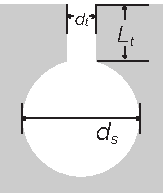
\includegraphics[height=1.25in]{print-and-play/blowhole/helmholtz_illustration}
        \quad
        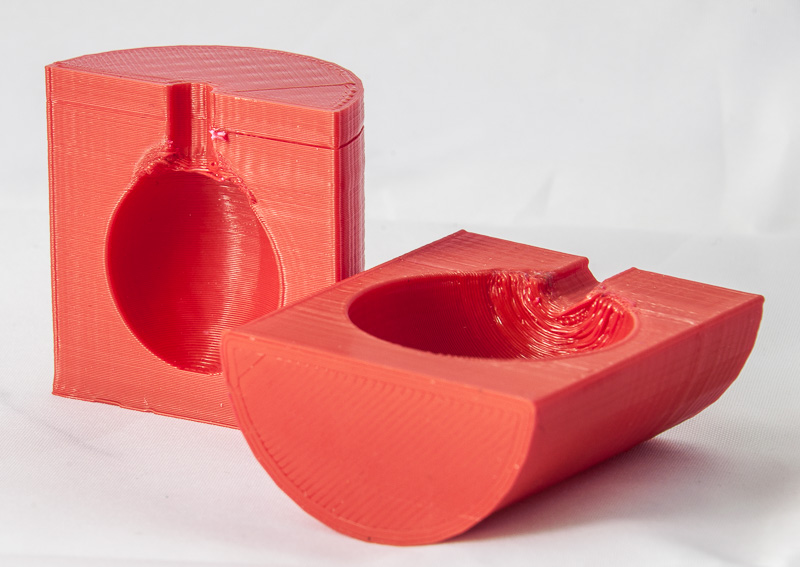
\includegraphics[height=1.25in]{print-and-play/blowhole/cavities2}
        \caption{Left: an ideal spherical Helmholtz resonator, with tube
          diameter $d_t$, tube length $L_t$, and sphere diameter $d_s$. Right:
          cross-sections of two \bh test objects, showing the resonator
          structures.}
        \label{fig:resonator}
      \end{figure}         

    \subsection{Blowhole Characterization} \label{sec:charac}
      In order for \bh to be of the most practical use, we want to understand
      how many different cavities we can fit inside a given object. As can be
      seen from Equation \ref{eq:hhz}, we can vary three parameters---$d_t, L_t$ or
      $d_s$---to change the resonant frequency of a \bh cavity. As the tube is
      the only user-facing element of \bh, its appearance should be consistent,
      with the size of the opening large enough to easily blow into, but not so
      large as to interfere with the features of the printed model. After some
      initial experimentation, we set $d_t$ to 5~mm, leaving $L_t$ and $d_s$ as
      the available parameters to manipulate. Multiple combinations of these can
      produce the same predicted frequency; for example, $L_t=2.5$~mm and
      $d_s=35.3$~mm produce a prediction of 1000~Hz, as do $L_t=5$~mm and
      $d_s=28$~mm.
      
      \begin{figure}
        \centering
        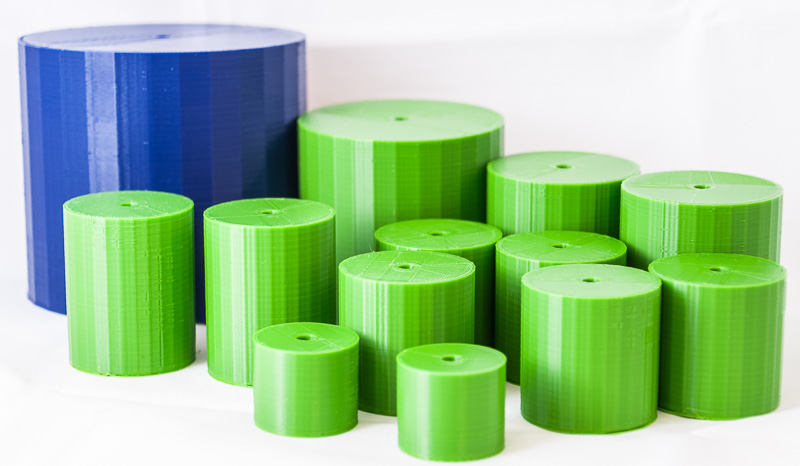
\includegraphics[width=.95\columnwidth]{print-and-play/blowhole/cylinders.jpg}
        \caption{A subset of our test cylinders with varying cavity volumes and
          tube lengths.}
        \label{fig:cylinders}
      \end{figure}
      
      To understand the practical limits on the frequencies we could detect and
      differentiate between, we produced a large number of test objects (Figure
      \ref{fig:cylinders}) using consumer FDM printers (Qidi Technology X-One,
      LulzBot Taz~4, and LulzBot Taz Mini). Wanting to understand the practical
      limits on the frequencies we could detect and differentiate between, we
      produced 48 objects with cavities and tubes of different sizes. Holding
      $d_t$ at 5~mm, we manipulated $d_s$ from 8--40~mm in steps of 4~mm and
      tested $L_t$ at 2.5, 3.5, 5, 7.5, 8.5 and 10~mm. These configurations
      gives us a frequency space ranging from 500~Hz, ($d_t=5$~mm, $L_t=10$~mm
      and $d_s=40$~mm) to 5900~Hz ($d_t=5$~mm, $L_t=2.5$~mm and $d_s=8$~mm).
          
      We asked ten people to blow into each cylinder between one and four times,
      recording the data via a laptop computer's built-in microphone at a
      44,100~Hz sampling rate. We extracted the fundamental frequencies of each
      blow using Welch's method \cite{Welch:1967jw}. Comparing the fundamental
      frequencies to the values predicted by the Helmholtz equation (Equation
      \ref{eq:hhz}), we find deviation, sometimes significant. However, the
      deviation is not constant, but presents as noise, with two main patterns:
      frequencies under 1000~Hz are much noisier than those higher; and longer
      tubes exhibit more noise than shorter. Figure \ref{fig:spectrogram}
      illustrates the spectrogram from one user for a series of blows into
      different cavity sizes.

      This behavior may be explained by several factors. First, the Helmholtz
      equation is a theoretical model known to be inexact for varying properties
      of cavity geometry \cite{Selamet:1995kv, Alster:1972ha}, assumes a
      reflective, smooth surface, and  as $L_t$ and $d_s$ approach 2--5\% of the
      resonant wavelength, the model begins to break down \cite{Selamet:1995kv}.
      As shown in Figure \ref{fig:resonator}, our 3D-printed models are not
      smooth. As the cavity size increases, the top of the sphere approaches
      horizontal, which can cause drooping or stringing. These features of 3D
      prints may affect the resonance. To validate print features as a potential
      cause, we printed eight duplicate test objects on a resin-based printer
      (the FormLabs Form~2), resulting in hard, smooth objects. Blows into these
      objects resulted in frequencies much closer to the predicted values.
      However, our goal is to maintain broad accessibility of our technique, so
      while noting the potential for resin printers to produce better results,
      we continue to describe our results using FDM printers.
      
      To validate the printability of our cavities, we tested multiple cavity
      sizes, from 5~mm to 60~mm in diameter. While all objects printed
      correctly, the smallest cylinders resulted in frequencies highly variable
      over the course of a single blow, and the 60~mm cavity failed to produce
      any strong harmonic at all.
      
      We also tested the consistency of sound at different angular positions of
      the tube opening, from 0° (straight down) to 180° (straight up) in 22.5°
      increments with $d_s$ as 16~mm and $L_t$ as 5~mm.  Although different
      orientations revealed different (minor) printing artifacts such as slight
      stringing and tube opening shape inconsistency, the results were
      consistent, with a mean deviation of under 240~Hz from the
      Helmholtz-predicted value.
      
      We tested \bh with multiple printers: a LulzBot Taz 4, a LulzBot Taz Mini,
      two Qidi X-One v2 printers, and a Form Labs Form~2 resin-based SLA
      printer. All printed successfully; inspecting the spectrograms, we found
      little variance amongst the FDM prints, and that the SLA prints produce
      dominant frequencies on average 100~Hz closer to the Helmholtz-predicted
      frequency than the FDM prints and with less variation over the signal.

  \section{System Implementation}
    As a system, \bh consists of three parts: the design software to modify
    existing 3D models to add blowholes; the physical printed-out models with
    resonant cavities and holes embedded; and the software that recognizes the
    sound of the user blowing into a cavity and performs an action. All
    pertinent code and designs can be found
    online~\footnote{\url{https://github.com/fetlab/blowhole-gi18}}.
          
    \subsection{Design Software}
      Our design software is built on top of Autodesk Meshmixer (Figure
      \ref{fig:software}, left) using its Python API for scripting remote
      command execution. To add \bh tags to a model, a user simply imports an
      existing model and then clicks on the model to specify tag locations and
      desired actions. Currently supported actions include opening URLs,
      launching files such as images and movies, and reading text via
      text-to-speech. After the user indicates all of their desired blowhole
      positions, the software determines the best set of cavity sizes to embed
      in the model. The na\"ive approach would be to simply place the largest
      possible available cavity in a location when the user selects it. However,
      this approach quickly fails; for example, if the user wished to place a
      blowhole in each eye of the elephant in Figure \ref{fig:elephant}, the
      first click would fill the elephant's head with a cavity and the second
      click would fail to find an acceptable cavity size. The opposite
      approach---choosing the smallest available size first---suffers from
      similar issues. 
      
      \begin{figure*}[t]
        \centering
        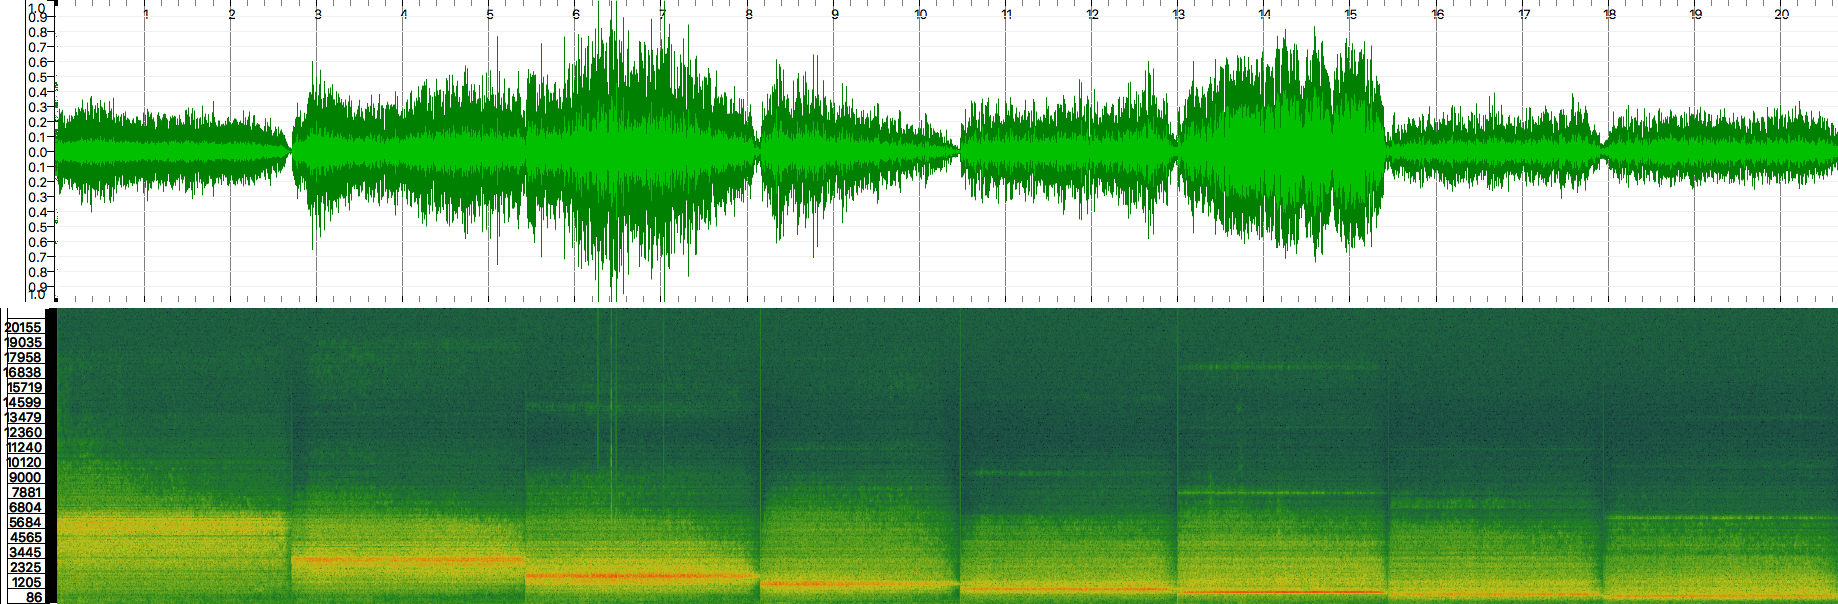
\includegraphics[width=\textwidth]{print-and-play/blowhole/spectrogram.png}
        \caption{Waveform (top) and spectrogram (bottom) of blows into holes with a tube length $L_t$ of 2.5~mm, with the cavity diameter $d_s$ varying in steps of 2~mm from 4~mm on the left to 18~mm on the right.}
        \label{fig:spectrogram}
      \end{figure*}

      Instead, our search algorithm allows the user to add all requested
      positions first, then attempts to optimize cavity placement by finding a
      set of $L_t$ and $d_s$ that will fit all requested blowhole locations
      without cavities colliding (we can optionally fix $L_t$ to a single
      value). The algorithm is based on depth-first search with backtracking. We
      represent the solution space---mapping a set of available cavities to
      desired blowhole positions---as a tree, with the root representing the
      original model, internal nodes as intermediate steps towards solutions,
      and leaves as final solutions. Each step of the algorithm takes as input a
      node, a list of candidate locations, and a list of unused cavity sizes. It
      tests each of the available cavities in the next candidate location until
      it finds one that fits within the model at that location. It then removes
      the candidate location and the cavity size from their respective lists and
      passes the newly modified model as a node to run the algorithm again. If,
      for a given node, no cavity can be found that fits within the candidate
      location, the tree is pruned at that point and the algorithm returns to
      the parent node to try the next child. When no candidate locations remain,
      we can output the current node's model as the solution; if candidate
      locations do remain but there are no more cavity sizes, we inform the user
      that we cannot find a solution. The search process takes under a minute.
          
      The final result is a set of location/cavity pairs, which we then use to
      construct the model for printing (Figure \ref{fig:software}, right). Once the
      cavities are placed, the software writes out a configuration file linking
      the cavity parameters $L_t$ and $d_s$ to the specified action. The final
      model may be exported to a STL file for 3D printing on a commodity
      printer.
          
      \begin{figure*}
        \centering
        \subfloat[]{\label{fig:sw1}
          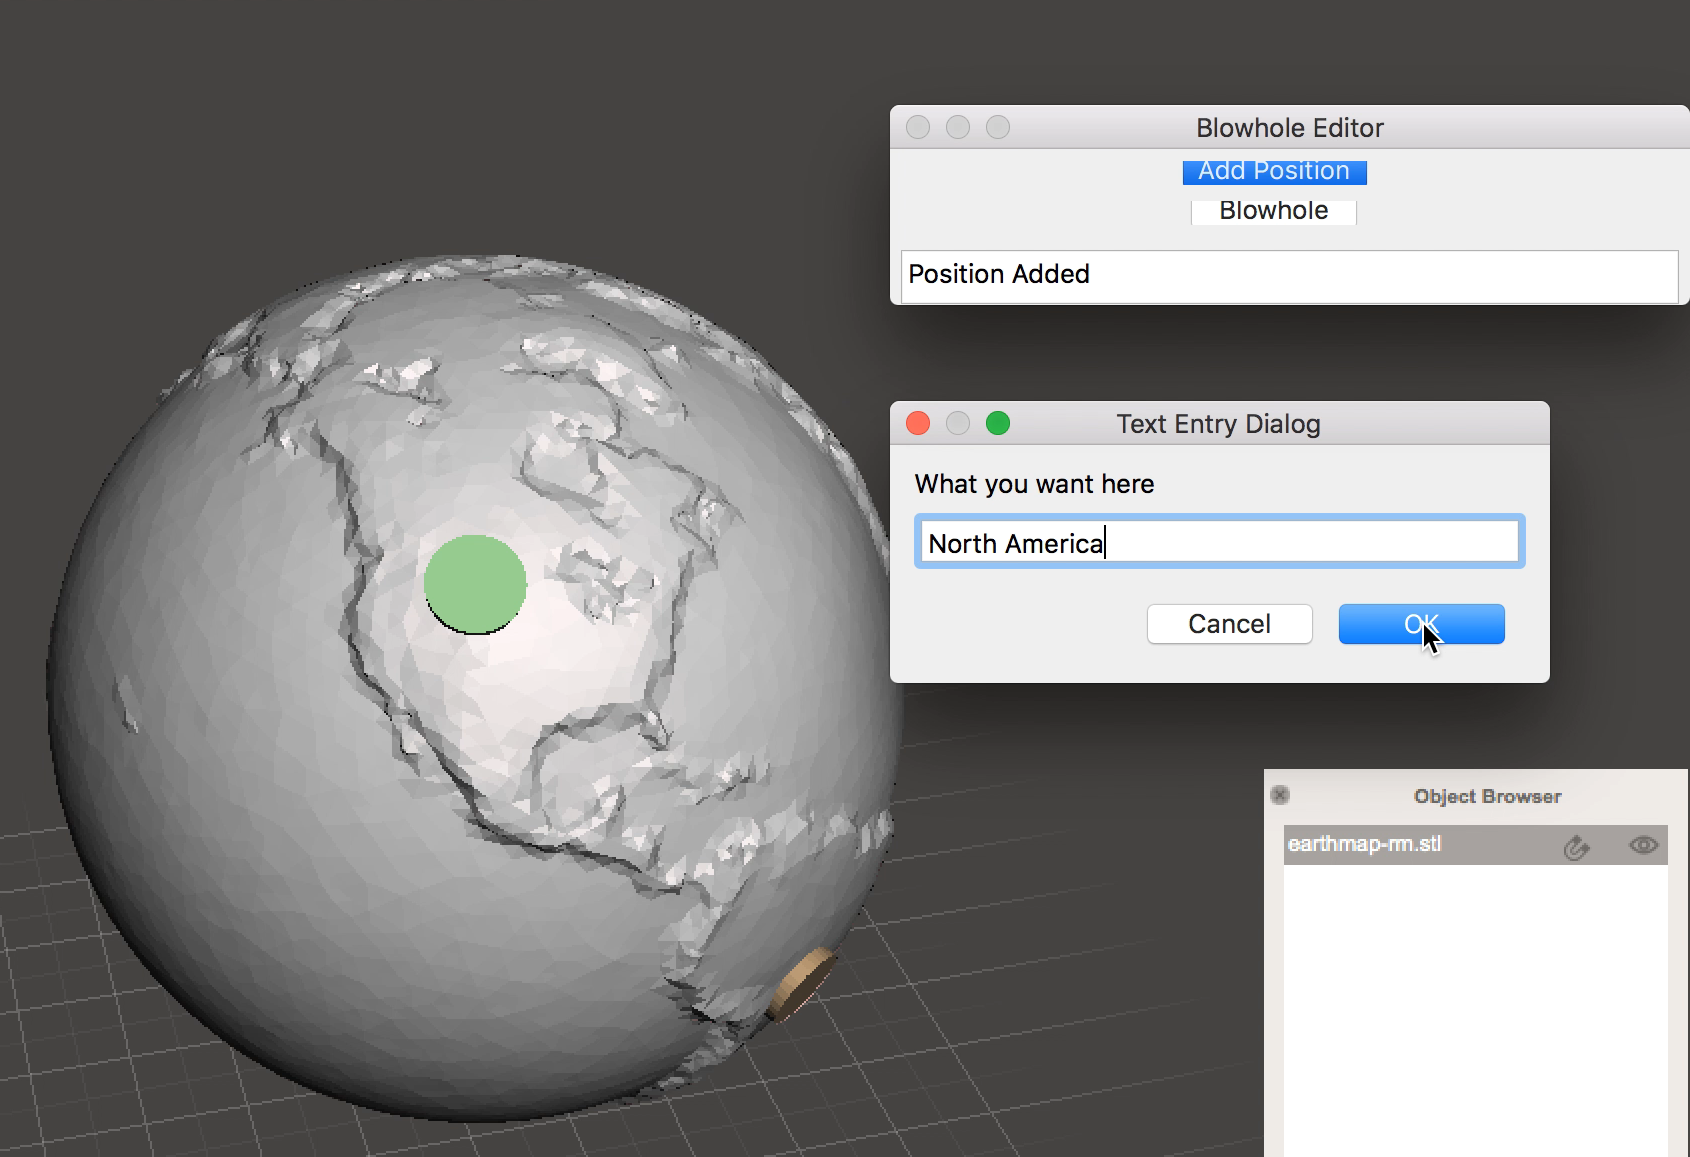
\includegraphics[height=.25\textwidth]{print-and-play/blowhole/mm_globe_full}}
        \qquad
        \subfloat[]{\label{fig:sw2}
          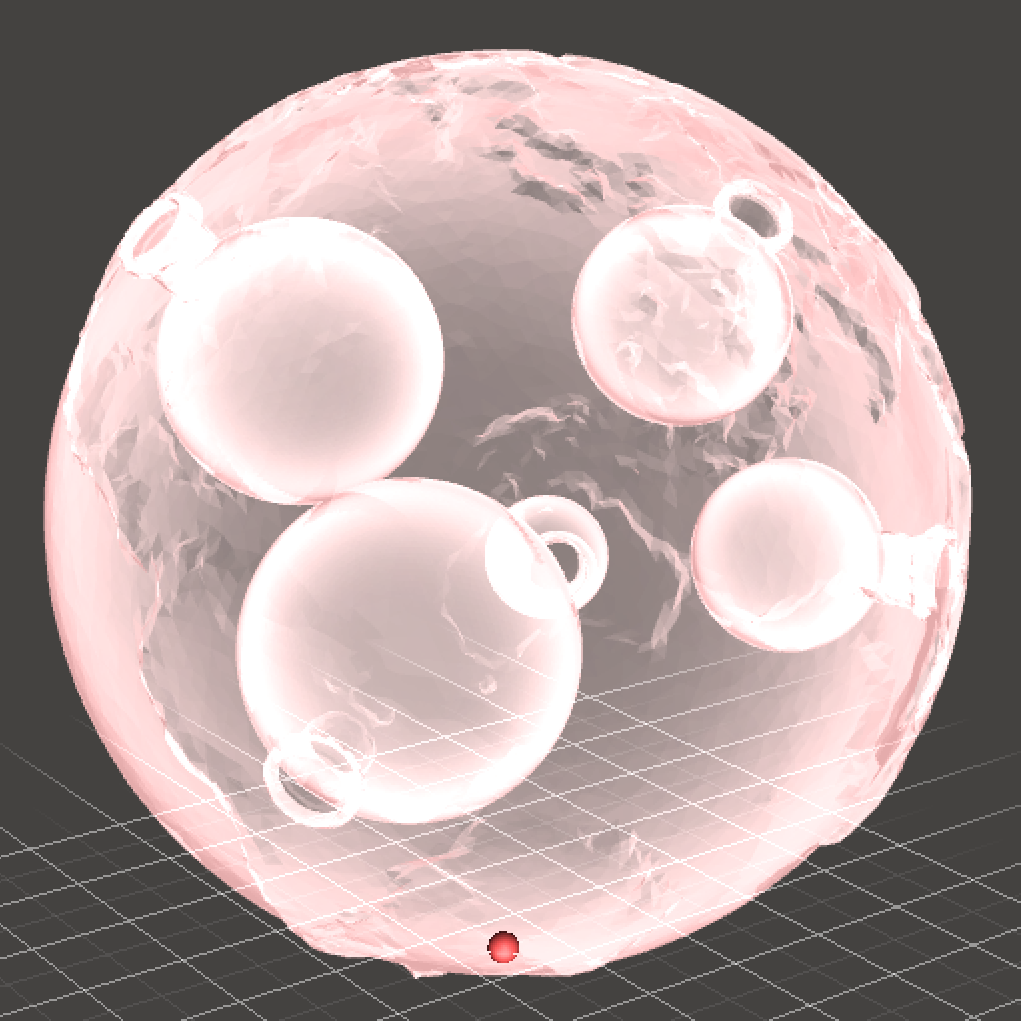
\includegraphics[height=.25\textwidth]{print-and-play/blowhole/mm_globe_trans}}
        \qquad
        \subfloat[]{\label{fig:globe}
          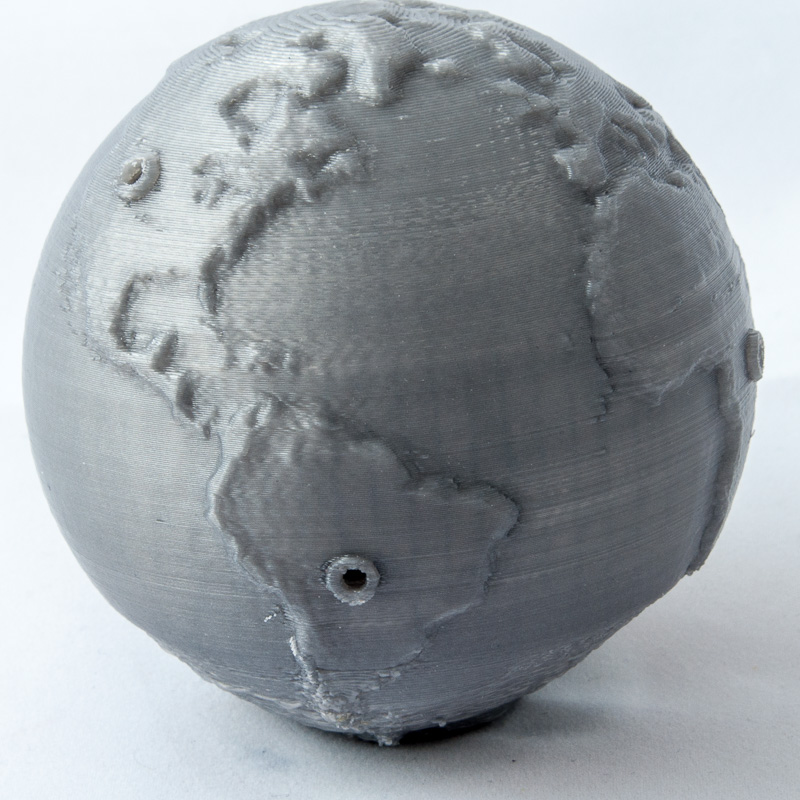
\includegraphics[height=.25\textwidth]{print-and-play/blowhole/globe04}}
        \caption{(\protect\subref*{fig:sw1},\protect\subref*{fig:sw2}):
        Detail view of our \bh design software, based on Meshmixer.
        \protect\subref{fig:sw1} shows the software with the user
        inserting blowholes: clicking a point on the model results
        in a placeholder (green dot) and a dialog box where the user
        can specify the action to be taken upon blowing.
        \protect\subref{fig:sw2} shows the interior of the model,
        illustrating the different-sized cavities the software
        inserted. \protect\subref{fig:globe} shows the final
        3D-printed object with blowholes embedded.}
        \label{fig:software}
      \end{figure*}
          
      In informal experiments with \bh-enabled objects, we found that locating
      the holes by feel alone could be challenging; on complex models like the
      elephant (Figure \ref{fig:elephant}) the hole gets ``lost'' in the model's
      geometry. Because one use scenario for \bh objects is as an aid for people
      with visual impairments, we added a ``ring'' feature. This simply adds a
      short (3 print layers, or about 0.64~mm high) ring extending 1~mm around
      the hole (Figure \ref{fig:blowhole_demo2}). In informal tests, we found
      that the ring is easily distinguishable by touch alone, allowing the hole
      to be easily located without vision. In order to avoid changing the sound
      produced, when we add the ring we shorten the inner end of the tube by the
      height of the ring, thereby maintaining the same $L_t$.
      
    \subsection{Blowhole Objects} 
      Our software places blowholes into existing models, therefore models that
      are 3D-printable will remain so with the addition of cavities and
      openings. Because the cavities are spherical, and most hobbyist-level 3D
      printers can print up to 45° of overhang, the models can be produced
      on most printers with no modification; importantly, no support material is
      necessary inside the cavities or tubes.
          
      Once a \bh-enabled object has been printed, some minor cleanup may be
      required: with larger spherical cavities, the top of the sphere becomes
      nearly horizontal, and the printer may produce some ``3D printer
      spaghetti'' (a small amount is visible in Figure \ref{fig:resonator}) that
      can slightly muffle the sound. A simple solution is to simply insert a
      drill bit of the appropriate size and twist it by hand to quickly remove
      the strands. 
          
      \begin{figure*}[t]
        \centering
        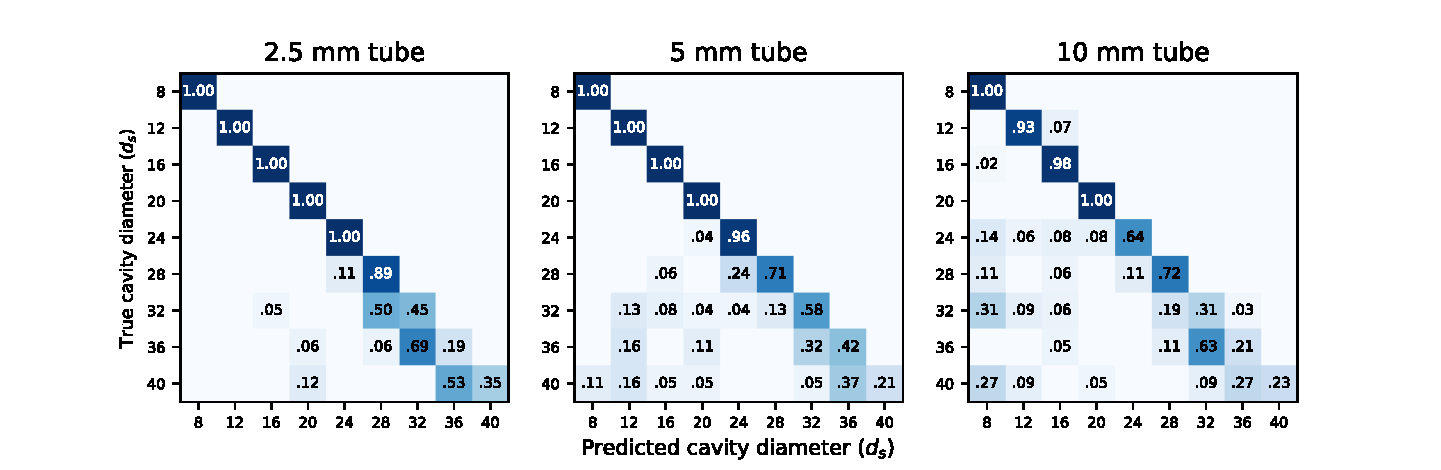
\includegraphics[width=.9\textwidth]{print-and-play/blowhole/tube_pct.pdf}
        \caption{Confusion matrices across all test participants for the three
          tested tube lengths with sphere diameters from 8--40~mm.}
        \label{fig:confusion}
      \end{figure*}
          
    \subsection{Blow Sound Recognition}
      The last component of our system recognizes the sounds produced by the
      user blowing into the blowholes, producing the resonant frequency
      characteristic to cavity/tube combinations (Figure \ref{eq:hhz}), allowing
      us to link the sound to the particular location the user is interacting
      with.  Our software is implemented in Python running on a laptop, but is
      simple enough to run on phones and smartwatches as well.

      To identify the resonant frequency, we window the 44,100~Hz incoming audio
      signal in 0.1s non-overlapping segments. We compute the RMS value of each
      and look for .5s worth of contiguous windows that exceed an empirically
      determined threshold. We apply Welch's method to extract the power
      spectrum of the signal \cite{Welch:1967jw}, and use the strongest
      frequency as the resonance. We then take the set of cavity/tube
      ($d_s/L_T$) combinations available and match the resonant frequency to the
      Helmholtz-predicted frequencies to determine which hole the user is
      interacting with. Once a blow is classified, the system executes the
      action referenced in the configuration file produced by the design
      software.
          
      Our main implementation is on a laptop computer, using its built-in
      microphone. We also tested with a LG-R Android smartwatch which transmits
      audio data to the same recognition pipeline. Our software runs in Python
      and uses the scikit-learn library for recognition.
          
    \subsection{Performance Testing}
      To validate our recognition procedure, we collected a total of 830 blow
      segments from ten participants as described in Section \ref{sec:charac},
      with $L_t$ of 2.5, 5, and 10~mm, and $d_s$ varying from 8--40~mm in 4~mm
      increments. We divided the data according to the tube length and evaluated
      our recognition procedure both overall and on a per-user basis.  Figure
      \ref{fig:confusion} presents a cross-validated evaluation of our
      classification system, where we can see that the reliability decreases as
      the diameter of the sphere increases.
          
      We found that as we include larger spheres and larger tubes, the
      recognition accuracy decreases. The best performance/versatility tradeoff
      occurs at $L_t$ of 2.5~mm and six spheres from 8--28~mm, which yields an
      overall 98\% accuracy. Adding a 32~mm sphere decreases accuracy to 90\%,
      and further spheres continue to decrease accuracy.

  \section{Examples}
    \begin{figure*}
        \centering
        \subfloat[]{\label{fig:rushmore}
            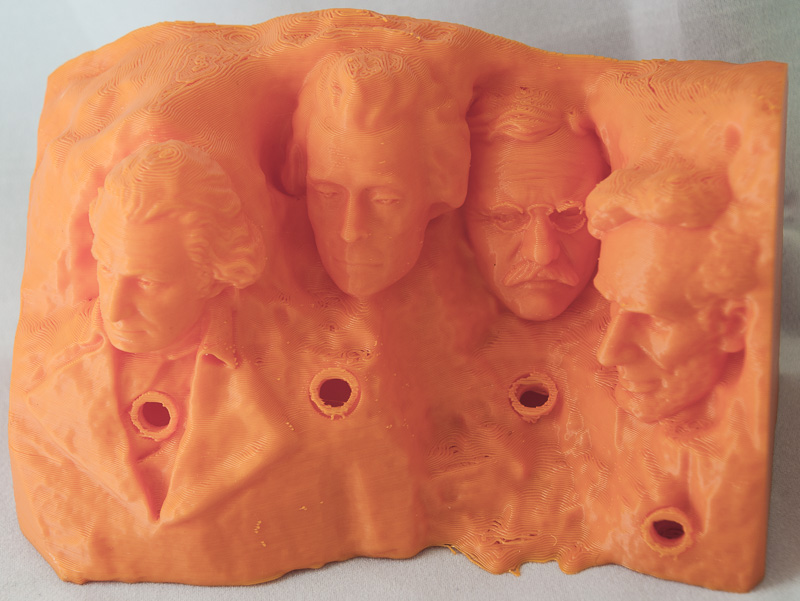
\includegraphics[height=.19\textwidth]{print-and-play/blowhole/rushmore}}
				\subfloat[]{\label{fig:bargraph2}
						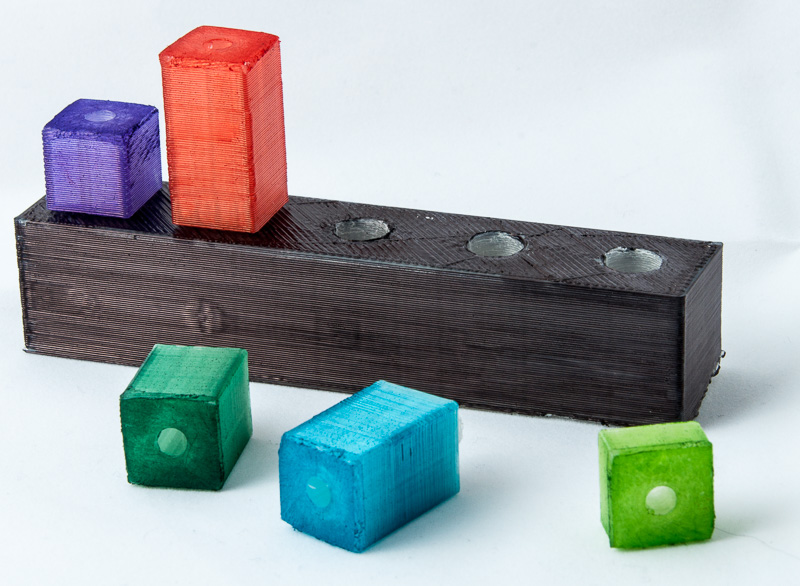
\includegraphics[height=.19\textwidth]{print-and-play/blowhole/bar_2in_3out}}
        \subfloat[]{\label{fig:musicbox}
            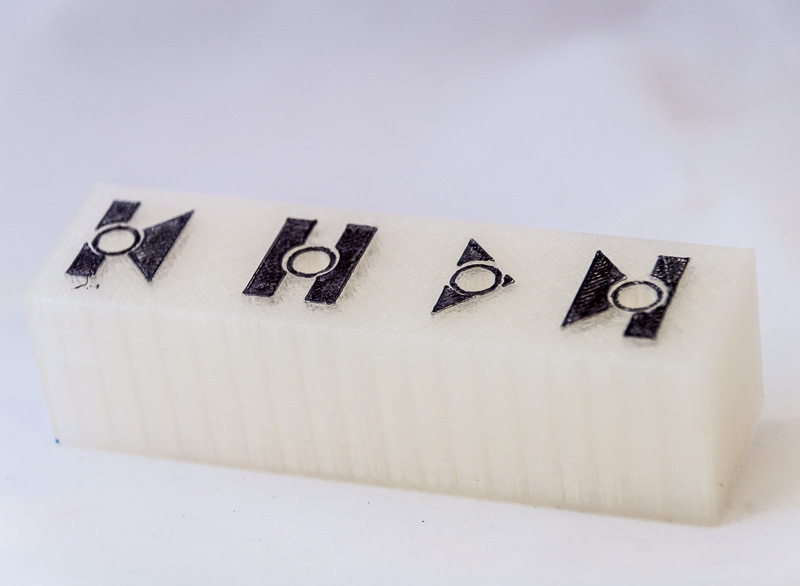
\includegraphics[height=.19\textwidth]{print-and-play/blowhole/music_box}}
        \subfloat[]{\label{fig:picturebook}
            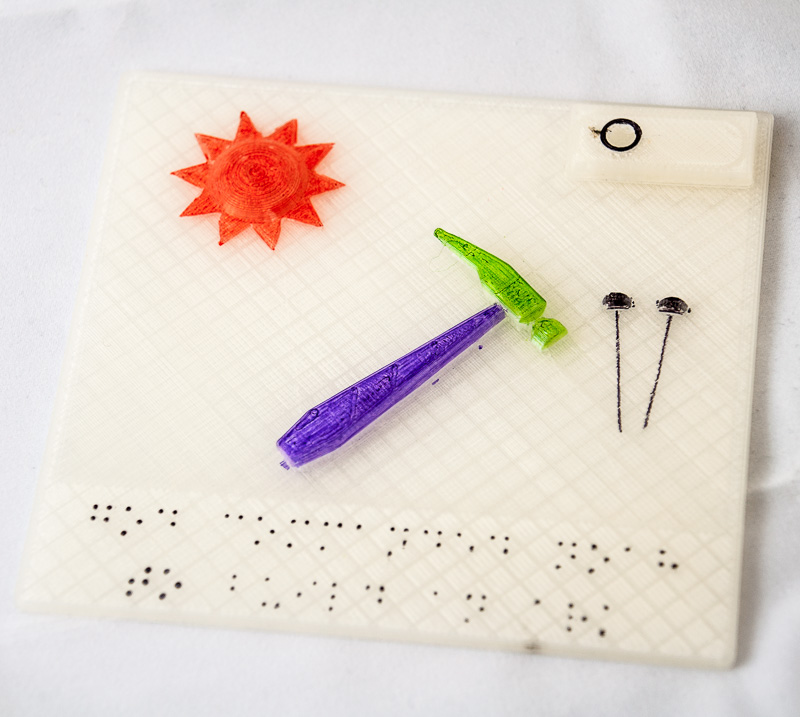
\includegraphics[height=.19\textwidth]{print-and-play/blowhole/book1}}
        \caption{Example \bh-augmented objects: \protect\subref{fig:rushmore} a
          model of Mt.~Rushmore with each president tagged;
          \protect\subref{fig:bargraph2} the bar graph from Figure
          \ref{fig:bar_rand} in a different arrangement;
          \protect\subref{fig:musicbox} a box that controls a music player by
          blowing; and \protect\subref{fig:picturebook} a 3D-printed tactile
          picture book for blind or low-vision children with a blowhole (upper
          right) which triggers text-to-speech of the Braille text.}
        \label{fig:blowhole_demo2}
    \end{figure*}

    To illustrate the potential of \bh, we present several possible
    applications. Each was built with our software and works with our
    recognition algorithm.
    
    \subsection*{Cell Model} 
      We adapted an existing model of an animal
      cell\footnote{\url{http://www.thingiverse.com/thing:689381}} to add \bh
      tags to the different parts of the cell (Figure \ref{fig:cell}). When the
      tags are activated, the listening computer application launches the
      Wikipedia page for the associated cell component.
        
    \subsection*{Globe} 
      Similar to the example in Tickers and Talker \cite{Shi:2016}, we tagged
      the continents on a 3d-printed
      globe\footnote{\url{http://www.thingiverse.com/thing:17336}} (Figure
      \ref{fig:globe}). When a user blows into the associated hole, our software
      speaks the name of the labeled continent using text-to-speech. 
    
    \subsection*{Interactive Animals} 
      We printed three different cetaceans: a
      dolphin\footnote{\url{http://www.thingiverse.com/thing:1121803}}, a
      whale\footnote{\url{http://www.thingiverse.com/thing:232247}}, and an
      orca\footnote{\url{http://www.thingiverse.com/thing:665571}}, and adapted
      the position of the cavity to the location of the animal's blowhole
      (Figure \ref{fig:whales}). When the user blows, the application plays a
      video about that animal.
    
    \subsection*{Music Controller}
      A ``music box'' with raised controls (Figure \ref{fig:musicbox}) allows a
      user to control the flow of music by blowing.  Each ``button'' has a
      different blowhole underneath it. Our segmentation algorithm described
      earlier is robust to background sound and in initial testing, its
      performance was not affected by the sound of the music playing.
    
    \subsection*{Augmented Tactile Book} 
      Previous research \cite{Kim:2015cva} has investigated 3D-printed tactile
      picture books for blind children. Some examples of these books have
      Braille text\footnote{\url{https://tactilepicturebooks.org/}}. We created
      a set of custom rectangular resonators, thinner than our standard \bh
      spherical resonators, to add to each page of a 3D-printed book (Figure
      \ref{fig:picturebook}). When the user blows into the hole, the computer
      reads aloud the text written in Braille on the page.
    
    \subsection*{Reconfigurable Bar Chart} 
      Figure \ref{fig:bar_rand} shows a \bh-enabled physical visualization
      \cite{Swaminathan:2014hu}. Taking advantage of the Helmholtz property that
      varying $L_t$ varies the frequency, the base of the bar chart contains
      cavities with identical $d_s$ values. Each bar, being a different height,
      has a different $L_t$; when a bar is plugged into the chart, the tone
      produced is due to the size of the bar. This characteristic enables
      reconfiguring the bar chart, illustrating data in different orders while
      maintaining the labels on the individual bars. Placing the resonating
      cavities in the base rather than the bars allows the bars to maintain
      smaller cross-sections but still produce audible tones.

  \section{Discussion and Future Work}
    Our goal with \bh was to create a system to enable non-experts to design and
    3D print interactive objects, with the particular aim of simplicity,
    avoiding interventions during printing, post-print processing, and complex
    training processes. \bh is usable for simple cases; with up to six cavities,
    the system achieves a high user-independent performance of 98\%. As
    illustrated by our examples in Figures \ref{fig:teaser}, and
    \ref{fig:blowhole_demo2}, six cavities are sufficient for many applications,
    and is a larger number of tags per object than have been demonstrated by
    other passive acoustic-based systems\cite{Reyes:2016, Li:2016, Shi:2016,
    Laput:2015, He:2017, Harrison:2012kw}.
    
    While \bh is successful, there is room for future improvement. We are
    interested in further characterizing the behavior of the cavities with
    different print settings; for example, we have encountered some tentative
    evidence that the type and amount of infill the printer uses to fill the
    solid parts of the model may have an effect on the sound. Refinements to the
    cavity shapes may also have an effect, for example by shaping the top of the
    spheres to avoid greater than 45° overhang in order to prevent the
    ``stringing'' effect. Additionally, we are interested in exploring the user
    experience while using this tool. We believe that tools like \bh can be
    particularly useful for educational settings, specially for children, due to
    its playfulness, as well as to enable new ways low vision users can interact
    with their technology. We will carry out user studies in the future to
    assess the experience of these two populations while using \bh.
    
  \section{Conclusion}
    We presented \bh, a system for adding acoustic ``tags'' to 3D-printed models
    via embedded cavities which resonate at characteristic frequencies when a
    user blows into them. Our system enables high performance for up to nine
    different blowholes, provides simple point-and-click design software, and
    \bh-enabled models are ready to use immediately post-printing with no
    assembly or external components required. We detailed the theory behind
    \bh's operation, presented our characterization of its performance, and
    demonstrated high user-dependent and -independent recognition rates. We
    demonstrated \bh's potential through multiple examples, including
    educational models, 3D-printed book pages, and a reconfigurable physical
    visualization. 